\documentclass[10pt]{beamer}  % Default is 11pt

\usetheme{Madrid}
\usecolortheme{default}
\usepackage[utf8]{inputenc}
\usepackage{amsmath}
\usepackage{amsfonts}
\usepackage{amssymb}
\usepackage{tikz}
\usepackage{xcolor}
\usepackage{hyperref}

\title{CRISC Exam - Hard Concepts \& Exam Traps}
\subtitle{Section 1: Risk Governance Deep Dive Tutorial}
\author{CRISC Mastery Series}
\date{\today}

\begin{document}
	
	% ============================================================
	% TITLE SLIDE
	% ============================================================
	\begin{frame}
		\titlepage
	\end{frame}
	
	% ============================================================
	% OUTLINE
	% ============================================================
	\begin{frame}{Section 1 Tutorial Outline}\   
		 \tiny
		\tableofcontents
	\end{frame}
	
	% ============================================================
	% SECTION 1: RISK GOVERNANCE - CORE CONCEPTS
	% ============================================================
	\section{1. Core Governance Concepts}
	
	% ----------------------------------------------------------------------
	\subsection{1.1 Governance vs Management}
	\begin{frame}{1.1 Governance vs Management - The Critical Distinction}
		\begin{block}{What is Governance?}
			\textbf{Governance} is the organizational framework that helps stakeholders set the \textbf{direction} and \textbf{alignment} with business objectives.
			\begin{itemize}
				\item Answers: "Are we doing the \textbf{right} things?"
				\item Answers: "Are these things done in the \textbf{right} way?"
				\item Provides \textbf{oversight} and \textbf{direction}
			\end{itemize}
		\end{block}
		
		\begin{alertblock}{The Critical Trap}
			Many candidates confuse \textbf{governance} with \textbf{management}. They are NOT the same!
		\end{alertblock}
		
		\begin{block}{What is Management?}
			\textbf{Management} focuses on \textbf{planning, building, executing, and monitoring}.
			\begin{itemize}
				\item Carries out the direction set by governance
				\item Reports results back to governance
				\item Focuses on \textbf{getting things done}
			\end{itemize}
		\end{block}
	\end{frame}
	
	\begin{frame}{1.1 Governance vs Management - Example}
		\begin{columns}
			\begin{column}{0.5\textwidth}
				\begin{block}{Governance Example}
					\begin{itemize}
						\item Board sets risk appetite
						\item Approves IT strategy
						\item Reviews security metrics
						\item Provides oversight
					\end{itemize}
					\vspace{0.3cm}
					\textbf{Who:} Board of Directors, Senior Management
				\end{block}
			\end{column}
			\begin{column}{0.5\textwidth}
				\begin{block}{Management Example}
					\begin{itemize}
						\item Implements security controls
						\item Executes risk assessments
						\item Manages day-to-day operations
						\item Reports to governance
					\end{itemize}
					\vspace{0.3cm}
					\textbf{Who:} CIO, CISO, IT Managers, Risk Managers
				\end{block}
			\end{column}
		\end{columns}
		
		\begin{exampleblock}{Key Takeaway}
			\centering
			\textbf{Governance = Direction and Oversight} \\
			\textbf{Management = Execution and Operations}
		\end{exampleblock}
	\end{frame}
	
	% ----------------------------------------------------------------------
	\subsection{1.2 The RACI Model}
	\begin{frame}{1.2 Understanding RACI}
		\begin{block}{RACI - Roles and Responsibilities}
			\begin{tabular}{|p{2cm}|p{3.5cm}|p{5cm}|}
				\hline
				\textbf{Role} & \textbf{Description} & \textbf{Example} \\
				\hline
				\textbf{Responsible} & Performs the work & Risk analyst conducts assessment \\
				\hline
				\textbf{Accountable} & Provides resources; final sign-off & CISO approves budget \\
				\hline
				\textbf{Consulted} & Subject matter experts & Business process owners \\
				\hline
				\textbf{Informed} & Kept updated & Board of Directors \\
				\hline
			\end{tabular}
		\end{block}
		
		\begin{alertblock}{The Critical Trap}
			\textbf{Accountable} and \textbf{Responsible} are often confused!
			\begin{itemize}
				\item \textbf{Responsible} = \textit{Does the work}
				\item \textbf{Accountable} = \textit{Owns the outcome}
			\end{itemize}
		\end{alertblock}
	\end{frame}
	
	% ----------------------------------------------------------------------
	\subsection{1.3 Risk Appetite, Tolerance, and Capacity}
	\begin{frame}{1.3 The Three Risk Concepts - Defined}
		\begin{block}{Critical Definitions}
			\begin{tabular}{|p{2.5cm}|p{8.5cm}|}
				\hline
				\textbf{Concept} & \textbf{Definition} \\
				\hline
				\textbf{Risk Appetite} & Amount of risk an organization is \textbf{willing to accept} in pursuit of its mission \\
				\hline
				\textbf{Risk Tolerance} & \textbf{Acceptable level of variation} from risk appetite for a specific risk \\
				\hline
				\textbf{Risk Capacity} & \textbf{Maximum risk} an organization can absorb before \textbf{existence is threatened} \\
				\hline
			\end{tabular}
		\end{block}
		
		\begin{alertblock}{The Critical Trap}
			\textbf{NEVER} confuse these three concepts in the exam!
		\end{alertblock}
		
		\begin{exampleblock}{Memory Aid}
			\begin{itemize}
				\item \textbf{Appetite} = \textit{"Willing to take"}
				\item \textbf{Tolerance} = \textit{"Acceptable deviation"}
				\item \textbf{Capacity} = \textit{"Can survive"}
			\end{itemize}
		\end{exampleblock}
	\end{frame}
	
	\begin{frame}{1.3 The Risk Hierarchy}
		\begin{center}
			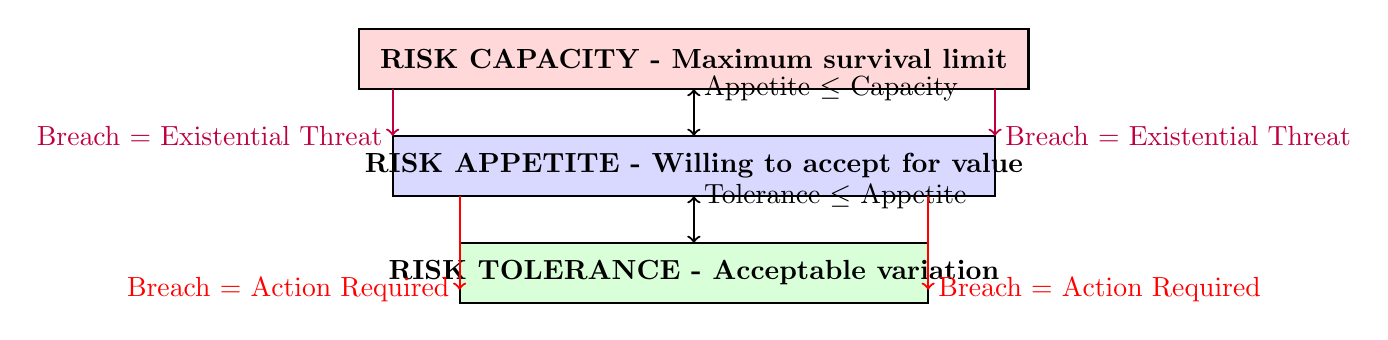
\begin{tikzpicture}[scale=0.85]
				% Capacity box - outermost
				\draw[thick, fill=red!15] (0,0) rectangle (10,0.9) node[midway] {\textbf{RISK CAPACITY - Maximum survival limit}};
				
				% Appetite box - middle
				\draw[thick, fill=blue!15] (0.5,-1.6) rectangle (9.5,-0.7) node[midway] {\textbf{RISK APPETITE - Willing to accept for value}};
				
				% Tolerance box - innermost
				\draw[thick, fill=green!15] (1.5,-3.2) rectangle (8.5,-2.3) node[midway] {\textbf{RISK TOLERANCE - Acceptable variation}};
				
				% Arrows showing relationship
				\draw[<->, thick] (5,-2.3) -- (5,-1.6) node[right] {Tolerance $\le$ Appetite};
				\draw[<->, thick] (5,-0.7) -- (5,0) node[right] {Appetite $\le$ Capacity};
				
				% Warning arrows
				\draw[->, thick, red] (1.5,-1.6) -- (1.5,-3.0) node[left] {Breach = Action Required};
				\draw[->, thick, red] (8.5,-1.6) -- (8.5,-3.0) node[right] {Breach = Action Required};
				
				\draw[->, thick, purple] (0.5,0) -- (0.5,-0.7) node[left] {Breach = Existential Threat};
				\draw[->, thick, purple] (9.5,0) -- (9.5,-0.7) node[right] {Breach = Existential Threat};
			\end{tikzpicture}
		\end{center}
	\end{frame}
	
	\begin{frame}{1.3 Understanding Risk Acceptance}
		\begin{block}{Risk Acceptance Process}
			\begin{itemize}
				\item Risk \textbf{within} risk appetite = Can be accepted
				\item Risk \textbf{within} risk tolerance = Can be accepted (with monitoring)
				\item Risk \textbf{above} risk tolerance = \textbf{MUST} take action
				\item Risk \textbf{above} risk capacity = \textbf{EXISTENTIAL THREAT}
			\end{itemize}
		\end{block}
		
		\begin{alertblock}{The Critical Trap}
			\textbf{Risk acceptance} does NOT mean ignoring risk!
			\begin{itemize}
				\item Must be \textbf{formally documented}
				\item Must be approved by \textbf{senior management}
				\item Must be \textbf{reviewed periodically}
				\item Must have \textbf{compensating controls} in place
			\end{itemize}
		\end{alertblock}
	\end{frame}
	
	% ----------------------------------------------------------------------
	\subsection{1.4 Common Exam Traps}
	\begin{frame}{1.4 Common Exam Traps - Risk Concepts}
		\begin{block}{Trap \#1: Appetite vs Tolerance}
			\begin{itemize}
				\item \textbf{Common Mistake}: Using "risk appetite" and "risk tolerance" interchangeably
				\item \textbf{Correct}: Appetite is \textbf{broad} organizational willingness; tolerance is \textbf{specific} acceptable deviation
				\item \textbf{Example}: Appetite = "We accept moderate risk for growth"; Tolerance = "15\% project cost overrun is acceptable"
			\end{itemize}
		\end{block}
		
		\begin{block}{Trap \#2: Tolerance vs Capacity}
			\begin{itemize}
				\item \textbf{Common Mistake}: Thinking tolerance breach is existential
				\item \textbf{Correct}: \textbf{Tolerance breach} requires management action; \textbf{Capacity breach} threatens existence
				\item \textbf{Example}: Projects exceed timeline by 15\% = tolerance; Bankruptcy = capacity
			\end{itemize}
		\end{block}
	\end{frame}
	
	% ============================================================
	% SECTION 2: RISK CULTURE AND COMMUNICATION
	% ============================================================
	\section{2. Risk Culture and Communication}
	
	% ----------------------------------------------------------------------
	\subsection{2.1 Understanding Risk Culture}
	\begin{frame}{2.1 What is Risk Culture?}
		\begin{block}{Risk Culture Defined}
			Risk culture represents the \textbf{shared values, attitudes, and behaviors} regarding risk management within an organization.
		\end{block}
		
		\begin{alertblock}{The Critical Insight}
			Organizational behavior has a \textbf{greater impact} on risk management effectiveness than any framework, tool, or policy!
		\end{alertblock}
		
		\begin{columns}
			\begin{column}{0.5\textwidth}
				\begin{block}{Healthy Risk Culture}
					\begin{itemize}
						\item Open communication
						\item Learning from failures
						\item Proactive escalation
						\item Accountability
						\item Transparency
					\end{itemize}
				\end{block}
			\end{column}
			\begin{column}{0.5\textwidth}
				\begin{block}{Toxic Risk Culture}
					\begin{itemize}
						\item Blame and finger-pointing
						\item Fear of reporting
						\item Hiding mistakes
						\item No accountability
						\item Cover-ups
					\end{itemize}
				\end{block}
			\end{column}
		\end{columns}
	\end{frame}
	
	\begin{frame}{2.2 The Blame Culture Phenomenon}
		\begin{block}{How Blame Culture Destroys Risk Management}
			\begin{itemize}
				\item People \textbf{hide mistakes} rather than report them
				\item No one \textbf{speaks up} about emerging risks
				\item Issues escalate until they become \textbf{major incidents}
				\item \textbf{Accountability is destroyed} - no one takes ownership
				\item \textbf{Root causes} are never identified or addressed
				\item Business units \textbf{point fingers} at IT when projects fail
			\end{itemize}
		\end{block}
		
		\begin{alertblock}{The Hard Truth}
			A blame culture is the \textbf{MOST effective inhibitor} of relevant and efficient communication in any organization.
		\end{alertblock}
	\end{frame}
	
	\begin{frame}{2.2 Risk Culture Maturity Levels}
		\begin{block}{Five Levels of Risk Culture}
			\begin{tabular}{|p{2cm}|p{3.5cm}|p{5.5cm}|}
				\hline
				\textbf{Level} & \textbf{Name} & \textbf{Characteristics} \\
				\hline
				1 & Vulnerable & No one cares; response is after incidents \\
				\hline
				2 & Reactive & Response based on complaints or compliance \\
				\hline
				3 & Compliant & Driven by external requirements only \\
				\hline
				4 & Proactive & Senior management supports risk management \\
				\hline
				5 & Resilient & Risk management is embedded in everything \\
				\hline
			\end{tabular}
		\end{block}
		
		\begin{exampleblock}{Critical Insight}
			\centering
			\Large{\textbf{Culture starts at the top!}}
			
			\normalsize{Senior management drives the culture of an organization. Without their support, risk management programs will almost always be unsuccessful.}
		\end{exampleblock}
	\end{frame}
	
	% ----------------------------------------------------------------------
	\subsection{2.3 Communication Inhibitors}
	\begin{frame}{2.3 The Communication Killers}
		\begin{block}{MOST Effective Inhibitor of Communication}
			\centering
			\Large{\textbf{BLAME CULTURE}}
		\end{block}
		
		\begin{block}{Other Inhibitors}
			\begin{itemize}
				\item \textbf{False sense of confidence} at top = consequence of poor communication
				\item \textbf{Perception of covering up} known risk = consequence of fear
				\item \textbf{Misalignment} between real risk appetite and policies = symptom of cultural issues
			\end{itemize}
		\end{block}
		
		\begin{exampleblock}{Key Takeaway}
			Address blame culture \textbf{FIRST} before implementing any risk management framework!
		\end{exampleblock}
	\end{frame}
	
	% ============================================================
	% SECTION 3: THREE LINES OF DEFENSE
	% ============================================================
	\section{3. Three Lines of Defense}
	
	% ----------------------------------------------------------------------
	\subsection{3.1 Understanding 3LoD}
	\begin{frame}{3.1 The Three Lines of Defense Model}
		\begin{block}{The 3LoD Framework}
			\begin{tabular}{|p{2.5cm}|p{3.5cm}|p{5cm}|}
				\hline
				\textbf{Line} & \textbf{Who} & \textbf{Primary Responsibility} \\
				\hline
				\textbf{1st Line} & Operational Management & Own and manage risk; implement controls \\
				\hline
				\textbf{2nd Line} & Risk Oversight Functions & Monitor, challenge, and provide guidance \\
				\hline
				\textbf{3rd Line} & Internal/External Audit & Provide independent assurance \\
				\hline
			\end{tabular}
		\end{block}
		
		\begin{alertblock}{The Critical Trap}
			Each line has \textbf{distinct, non-overlapping responsibilities}. Confusing these roles is a \textbf{major exam trap}!
		\end{alertblock}
		
		\begin{exampleblock}{Memory Aid}
			\begin{itemize}
				\item \textbf{1st Line = "Do It"}
				\item \textbf{2nd Line = "Watch It"}
				\item \textbf{3rd Line = "Check It"}
			\end{itemize}
		\end{exampleblock}
	\end{frame}
	
	\begin{frame}{3.1 Detailed Responsibilities}
		\begin{block}{First Line - Operational Management}
			\begin{itemize}
				\item Business owners with thorough understanding of business
				\item Responsible for implementing risk management practices
				\item Responsible for internal control monitoring
				\item Ensure control deficiencies are highlighted and addressed
				\item \textbf{ULTIMATE RISK OWNERS}
			\end{itemize}
		\end{block}
		
		\begin{block}{Second Line - Risk and Compliance Functions}
			\begin{itemize}
				\item Develop risk management framework and policy documentation
				\item Communicate framework across the organization
				\item Monitor first line activities for compliance
				\item Develop \textbf{KRIs} and keep stakeholders informed
			\end{itemize}
		\end{block}
	\end{frame}
	
	\begin{frame}{3.1 Third Line - Audit}
		\begin{block}{Third Line - Internal/External Audit}
			\begin{itemize}
				\item \textbf{Independence} is the most important aspect
				\item Evaluate effectiveness of first and second line activities
				\item Provide \textbf{independent opinions} on conformance
				\item Report findings to audit committee/board
			\end{itemize}
		\end{block}
		
		\begin{alertblock}{The Critical Trap}
			\textbf{Independence} is the KEY requirement for the third line!
			\begin{itemize}
				\item Cannot be involved in designing controls
				\item Cannot be involved in implementing controls
				\item Cannot report to the same management they audit
			\end{itemize}
		\end{alertblock}
	\end{frame}
	
	% ----------------------------------------------------------------------
	\subsection{3.2 Common 3LoD Traps}
	\begin{frame}{3.2 Common 3LoD Exam Traps}
		\begin{block}{Trap \#1: Who Owns Risk?}
			\begin{itemize}
				\item \textbf{Common Mistake}: Thinking IT owns technology risk
				\item \textbf{Correct}: \textbf{Business management} owns all risk
				\item \textbf{Why}: Risk impacts business objectives; IT is an enabler
			\end{itemize}
		\end{block}
		
		\begin{block}{Trap \#2: Who Establishes Framework?}
			\begin{itemize}
				\item \textbf{Common Mistake}: Thinking internal audit establishes risk framework
				\item \textbf{Correct}: \textbf{Second Line} establishes and maintains framework
				\item \textbf{Why}: Framework is an oversight function, not assurance function
			\end{itemize}
		\end{block}
		
		\begin{block}{Trap \#3: Who Tests Controls?}
			\begin{itemize}
				\item \textbf{Common Mistake}: Thinking first line tests controls
				\item \textbf{Correct}: \textbf{Third line} (audit) tests control effectiveness
				\item \textbf{Why}: Independence is required for objective testing
			\end{itemize}
		\end{block}
	\end{frame}
	
	% ============================================================
	% SECTION 4: POLICY DOCUMENTATION
	% ============================================================
	\section{4. Policy Documentation Hierarchy}
	
	% ----------------------------------------------------------------------
	\subsection{4.1 Understanding the Hierarchy}
	\begin{frame}{4.1 Policy Documentation Hierarchy}
		\begin{center}
			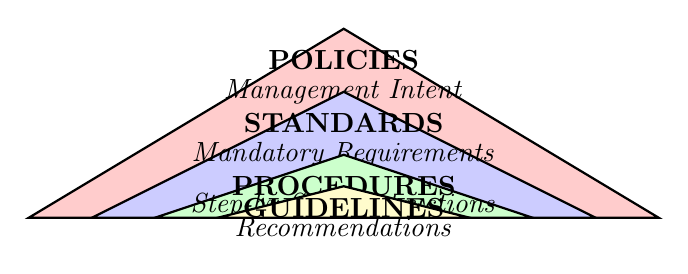
\begin{tikzpicture}[scale=0.8]
				% Pyramid shape
				\draw[thick, fill=red!20] (0,0) -- (10,0) -- (5,3) -- cycle;
				\node at (5,2.5) {\textbf{POLICIES}};
				\node at (5,2.0) {\textit{Management Intent}};
				
				\draw[thick, fill=blue!20] (1,0) -- (9,0) -- (5,2) -- cycle;
				\node at (5,1.5) {\textbf{STANDARDS}};
				\node at (5,1.0) {\textit{Mandatory Requirements}};
				
				\draw[thick, fill=green!20] (2,0) -- (8,0) -- (5,1) -- cycle;
				\node at (5,0.5) {\textbf{PROCEDURES}};
				\node at (5,0.2) {\textit{Step-by-Step Instructions}};
				
				\draw[thick, fill=yellow!20] (3,0) -- (7,0) -- (5,0.5) -- cycle;
				\node at (5,0.15) {\textbf{GUIDELINES}};
				\node at (5,-0.15) {\textit{Recommendations}};
			\end{tikzpicture}
		\end{center}
		
		\begin{exampleblock}{Memory Aid}
			\begin{itemize}
				\item \textbf{Policies} = \textit{"What" we do}
				\item \textbf{Standards} = \textit{"How" we do it}
				\item \textbf{Procedures} = \textit{"Step-by-step" instructions}
				\item \textbf{Guidelines} = \textit{"Recommendations" for best practices}
			\end{itemize}
		\end{exampleblock}
	\end{frame}
	
	\begin{frame}{4.1 Detailed Definitions}
		\begin{block}{Policies}
			\begin{itemize}
				\item High-level statements of \textbf{management intent}
				\item Designed to \textbf{influence decisions}
				\item Guide the organization to achieve desired outcomes
				\item \textbf{Business decision}, NOT a technical one
			\end{itemize}
		\end{block}
		
		\begin{block}{Standards}
			\begin{itemize}
				\item \textbf{Mandatory} requirements
				\item Granular and prescriptive
				\item Establish minimum security requirements
				\item Ensure systems include appropriate protections
			\end{itemize}
		\end{block}
	\end{frame}
	
	\begin{frame}{4.1 Procedures and Guidelines}
		\begin{block}{Procedures}
			\begin{itemize}
				\item Documented set of \textbf{steps} to perform a task
				\item Answer: "How do we operationalize the policy?"
				\item Provide \textbf{defendable evidence} of due care
				\item Also called \textbf{SOPs} (Standard Operating Procedures)
			\end{itemize}
		\end{block}
		
		\begin{block}{Guidelines}
			\begin{itemize}
				\item \textbf{Recommended practices}
				\item Based on industry-recognized secure practices
				\item Allow \textbf{discretion} or \textbf{leeway}
				\item Augment standards when discretion is permissible
			\end{itemize}
		\end{block}
	\end{frame}
	
	\begin{frame}{4.1 Example - Encryption}
		\begin{block}{Example: Implementing Encryption}
			\begin{tabular}{|p{2.5cm}|p{8.5cm}|}
				\hline
				\textbf{Document} & \textbf{Content} \\
				\hline
				Policy & "Employees should encrypt all data at rest" \\
				\hline
				Standard & "Use AES-256 encryption algorithm" \\
				\hline
				Procedure & "Step-by-step guide on how to encrypt data" \\
				\hline
				Guideline & "What to do if encryption fails" \\
				\hline
			\end{tabular}
		\end{block}
		
		\begin{alertblock}{The Critical Trap}
			Policies are \textbf{HIGH-LEVEL} and \textbf{NON-TECHNICAL}. \\
			Procedures are \textbf{DETAILED} and \textbf{TECHNICAL}.
		\end{alertblock}
	\end{frame}
	
	% ----------------------------------------------------------------------
	\subsection{4.2 Essential Policies}
	\begin{frame}{4.2 Essential Policies for Risk Management}
		\begin{block}{Must-Have Policies}
			\begin{itemize}
				\item \textbf{Information Security Policy} - Foundation for all controls
				\item \textbf{Access Control Policy} - Authentication, authorization, removal
				\item \textbf{Data Classification Policy} - Security based on sensitivity
				\item \textbf{Password Policy} - Length, complexity, expiration
				\item \textbf{Acceptable Use Policy} - Use of company resources
				\item \textbf{Backup Policy} - Frequency and extent of backups
			\end{itemize}
		\end{block}
		
		\begin{block}{Additional Key Policies}
			\begin{itemize}
				\item Logging and Monitoring Policy
				\item Risk Assessment Policy
				\item Change Management Policy
				\item Incident Response Policy
				\item Business Continuity Plan
			\end{itemize}
		\end{block}
	\end{frame}
	
	\begin{frame}{4.2 Policy Review Requirements}
		\begin{block}{Policy Review Best Practices}
			\begin{itemize}
				\item Review and approve at least \textbf{ANNUALLY}
				\item Review after \textbf{MAJOR} changes in business process
				\item Review after \textbf{INFRASTRUCTURE} changes
				\item Ensure policies still support \textbf{management's intent}
			\end{itemize}
		\end{block}
		
		\begin{alertblock}{The Critical Trap}
			\begin{itemize}
				\item \textbf{Incorrect}: Policies only need review when "something happens"
				\item \textbf{Correct}: Policies must be reviewed \textbf{systematically}, at minimum annually
				\item \textbf{Why}: Threats and business environment change constantly
			\end{itemize}
		\end{alertblock}
	\end{frame}
	
	% ============================================================
	% SECTION 5: ASSET MANAGEMENT
	% ============================================================
	\section{5. Asset Management}
	
	% ----------------------------------------------------------------------
	\subsection{5.1 Understanding Assets}
	\begin{frame}{5.1 Asset Identification}
		\begin{block}{The Golden Rule}
			\centering
			\Large{\textbf{"You can't protect what you don't know exists."}}
		\end{block}
		
		\begin{block}{Major Asset Categories}
			\begin{tabular}{|p{2.5cm}|p{4cm}|p{4.5cm}|}
				\hline
				\textbf{Asset Type} & \textbf{Examples} & \textbf{Risk} \\
				\hline
				\textbf{People} & Employees, contractors & Key person dependency \\
				\hline
				\textbf{Technology} & Systems, networks, laptops & Outdated systems, unpatched \\
				\hline
				\textbf{Data} & Customer data, IP, financials & Breach, loss, corruption \\
				\hline
				\textbf{IP} & Patents, trade secrets, copyrights & Loss of competitive advantage \\
				\hline
			\end{tabular}
		\end{block}
	\end{frame}
	
	% ----------------------------------------------------------------------
	\subsection{5.2 Data Classification}
	\begin{frame}{5.2 Data Classification and Labeling}
		\begin{block}{Why Classify Data?}
			\begin{itemize}
				\item Determines \textbf{sensitivity} of data
				\item Defines \textbf{controls} required to keep it secure
				\item \textbf{Directly impacts} cost of controls
				\item Enables \textbf{appropriate protection}
			\end{itemize}
		\end{block}
		
		\begin{block}{Classification Factors}
			\begin{itemize}
				\item \textbf{Regulatory requirements} - HIPAA, GDPR, PCI-DSS
				\item \textbf{Business impact} - Critical vs Public
				\item \textbf{Type} - PII, financial, health records
				\item \textbf{Access control} - Restricted vs Public
				\item \textbf{Location} - On-premises vs Cloud
			\end{itemize}
		\end{block}
	\end{frame}
	
	\begin{frame}{5.2 Data Owner vs Custodian}
		\begin{block}{Critical Role Distinction}
			\begin{tabular}{|p{2.5cm}|p{4cm}|p{4.5cm}|}
				\hline
				\textbf{Role} & \textbf{Responsibility} & \textbf{Example} \\
				\hline
				\textbf{Data Owner} & \textit{Decides} what happens & Classifies data; approves access \\
				\hline
				\textbf{Data Custodian} & \textit{Implements} controls & Backup; encryption; patching \\
				\hline
				\textbf{Data User} & \textit{Uses} data & Reads/updates authorized data \\
				\hline
			\end{tabular}
		\end{block}
		
		\begin{alertblock}{The Critical Trap}
			\textbf{Common Mistake}: Thinking IT classifies data.
			
			\textbf{Correct}: The \textbf{DATA OWNER} classifies data based on business criticality.
			
			\textbf{Why}: IT doesn't know the business value of the data.
		\end{alertblock}
	\end{frame}
	
	% ============================================================
	% SECTION 6: COMMANDMENTS AND KEY TAKEAWAYS
	% ============================================================
	\section{6. The 10 Commandments of Risk Governance}
	
	% ----------------------------------------------------------------------
	\subsection{6.1 The 10 Commandments}
	\begin{frame}{6.1 The 10 Commandments of Risk Governance}
		\begin{block}{Commandment 1}
			\centering
			\textbf{Thou shalt know the difference between Governance and Management}
		\end{block}
		
		\begin{block}{Commandment 2}
			\centering
			\textbf{Thou shalt NEVER confuse Risk Appetite, Tolerance, and Capacity}
		\end{block}
		
		\begin{block}{Commandment 3}
			\centering
			\textbf{Thou shalt understand that Business owns Risk, NOT IT}
		\end{block}
		
		\begin{block}{Commandment 4}
			\centering
			\textbf{Thou shalt address Blame Culture before implementing any framework}
		\end{block}
	\end{frame}
	
	\begin{frame}{6.1 The 10 Commandments (Continued)}
		\begin{block}{Commandment 5}
			\centering
			\textbf{Thou shalt know the 3 Lines of Defense: Do, Watch, Check}
		\end{block}
		
		\begin{block}{Commandment 6}
			\centering
			\textbf{Thou shalt recognize that Policies = Intent, Procedures = Steps}
		\end{block}
		
		\begin{block}{Commandment 7}
			\centering
			\textbf{Thou shalt know that Data Owners Classify, Custodians Implement}
		\end{block}
		
		\begin{block}{Commandment 8}
			\centering
			\textbf{Thou shalt document Risk Acceptance with Senior Management sign-off}
		\end{block}
	\end{frame}
	
	\begin{frame}{6.1 The 10 Commandments (Continued)}
		\begin{block}{Commandment 9}
			\centering
			\textbf{Thou shalt review Policies at minimum ANNUALLY}
		\end{block}
		
		\begin{block}{Commandment 10}
			\centering
			\textbf{Thou shalt align Risk Management with Business Objectives}
		\end{block}
	\end{frame}
	
	% ----------------------------------------------------------------------
	\subsection{6.2 Final Exam Tips}
	\begin{frame}{6.2 Final Exam Tips - Governance}
		\begin{block}{Governance Section Success Strategy}
			\begin{itemize}
				\item \textbf{Remember the Hierarchy}: Board > Senior Management > Managers > Staff
				\item \textbf{Think "Business First"}: Always align with business objectives
				\item \textbf{Know Your Definitions}: Use ISACA definitions, not general ones
				\item \textbf{Look for "MOST"}: ISACA wants the \textit{primary} answer
				\item \textbf{Culture Matters}: Always consider organizational culture
			\end{itemize}
		\end{block}
		
		\begin{exampleblock}{The ISACA Mindset for Governance}
			\centering
			\Large{\textbf{Governance = Direction and Oversight}}
			
			\normalsize{When in doubt, ask: "Who provides oversight and sets direction?"}
		\end{exampleblock}
	\end{frame}
	
	\begin{frame}{6.2 Quick Reference Card}
		\begin{block}{Risk Governance - Quick Reference}
			\begin{tabular}{|p{3.5cm}|p{3cm}|p{3.5cm}|}
				\hline
				\textbf{Concept} & \textbf{Definition} & \textbf{Example} \\
				\hline
				Governance & Direction \& Oversight & Board sets strategy \\
				\hline
				Management & Execution \& Operations & IT implements controls \\
				\hline
				Risk Appetite & Willing to accept & "Moderate risk for growth" \\
				\hline
				Risk Tolerance & Acceptable variation & "15\% cost overrun allowed" \\
				\hline
				Risk Capacity & Maximum survival & "Can absorb \$50M loss" \\
				\hline
				1st LoD & Operational Mgmt & Risk owners \\
				\hline
				2nd LoD & Risk Oversight & Risk management \\
				\hline
				3rd LoD & Audit & Internal/External audit \\
				\hline
			\end{tabular}
		\end{block}
	\end{frame}
	
	\begin{frame}{Final Advice}
		\begin{block}{Section 1 - Risk Governance}
			\centering
			\vspace{0.3cm}
			\textbf{Remember:}
			\begin{itemize}
				\item Governance provides \textbf{direction} and \textbf{oversight}
				\item Management \textbf{executes} and \textbf{operates}
				\item Risk \textbf{Appetite} $\ne$ Risk \textbf{Tolerance} $\ne$ Risk \textbf{Capacity}
				\item 3 Lines = \textbf{Do}, \textbf{Watch}, \textbf{Check}
				\item Policies = \textbf{Intent}, Procedures = \textbf{Steps}
				\item \textbf{Culture} matters more than any framework
			\end{itemize}
			\vspace{0.5cm}
			\textbf{Next: Section 2 - IT Risk Assessment}
		\end{block}
	\end{frame}
	
	% ============================================================
	% END OF PRESENTATION
	% ============================================================
	
\end{document}